\documentclass[10pt,letterpaper]{article}
\usepackage[margin=0.95in]{geometry}
\usepackage{booktabs}
\usepackage{array}
\newcolumntype{L}[1]{>{\raggedright\arraybackslash}p{#1}}
\usepackage{tikz}
\usetikzlibrary{arrows.meta,positioning,fit,calc,backgrounds}
\usepackage{enumitem}
\usepackage{amsmath}
\usepackage[hidelinks]{hyperref}
\usepackage[T1]{fontenc}
\setlist{nosep,leftmargin=*}
\setlength{\parskip}{4pt}
\setlength{\parindent}{0pt}
\setlength{\emergencystretch}{2em}

\title{\vspace{-1.2em}A measurement-based study of physical AI inference\\[2pt]\large Working notes: setup, facets, and evidence base}
\author{P.\ (Columbia)}
\date{September 22, 2026}

\begin{document}
\maketitle
\vspace{-1.5em}

\section{Thesis and shape of the study}

Physical AI inference (VLAs, world models, and the runtimes around them) is an autoregressive generator feeding a fixed-rate consumer through a stale input channel. The generator emits chunks (action chunks, video blocks); the consumer runs on a clock (actuator loop, display); the input (camera, control events) is always older than the moment the output takes effect. Every published mitigation (RTC, TT-RTC, VLASH, A2C2) is an ML fix for one symptom of that structure, and every published evaluation injects latency as a fixed integer instead of measuring it.

The hypothesis to test: \textbf{physical AI inference fails at the interfaces between layers, not inside the model.} Workload$\leftrightarrow$model is staleness; non-model load$\leftrightarrow$model is contention; model$\leftrightarrow$device is transport. If that holds, the fix is a runtime, not another training augmentation.

The study is a measurement grid. Each cell is a configuration of the stack below; each cell yields a failure classification and a task-quality number.

\subsection{The stack}

\begin{center}
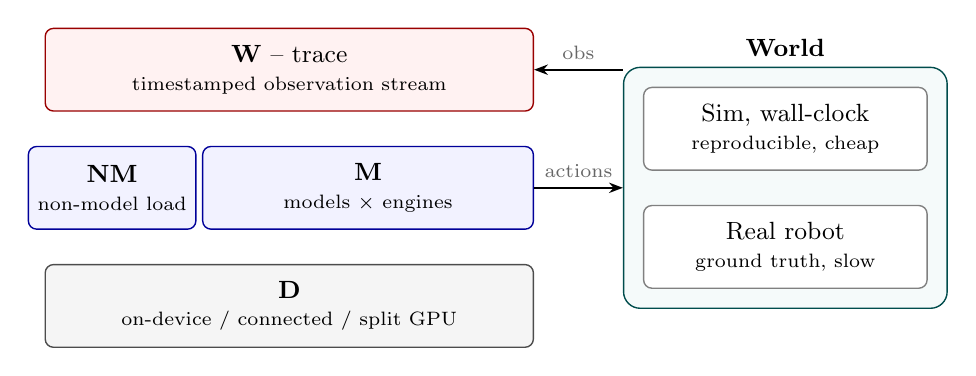
\begin{tikzpicture}[
  every node/.style={font=\small},
  blk/.style={draw,rounded corners=3pt,minimum height=1.05cm,align=center,line width=0.5pt},
  lbl/.style={font=\scriptsize,text=black!60}
]
  \node[blk,minimum width=6.2cm,fill=red!5,draw=red!60!black]   (W)  at (0,3.0)  {\textbf{W} -- trace\\[-1pt]{\scriptsize timestamped observation stream}};
  \node[blk,minimum width=1.7cm,fill=blue!5,draw=blue!60!black] (NM) at (-2.25,1.5) {\textbf{NM}\\[-1pt]{\scriptsize non-model load}};
  \node[blk,minimum width=4.2cm,fill=blue!5,draw=blue!60!black] (M)  at (1.0,1.5)  {\textbf{M}\\[-1pt]{\scriptsize models $\times$ engines}};
  \node[blk,minimum width=6.2cm,fill=black!4,draw=black!70]     (D)  at (0,0)    {\textbf{D}\\[-1pt]{\scriptsize on-device / connected / split GPU}};

  \node[blk,minimum width=3.6cm,fill=white,draw=black!50] (SIM) at (6.3,2.25) {Sim, wall-clock\\[-1pt]{\scriptsize reproducible, cheap}};
  \node[blk,minimum width=3.6cm,fill=white,draw=black!50] (ROB) at (6.3,0.75) {Real robot\\[-1pt]{\scriptsize ground truth, slow}};
  \begin{scope}[on background layer]\node[draw=teal!60!black,rounded corners=6pt,fit=(SIM)(ROB),inner sep=7pt,fill=teal!4,line width=0.5pt] (WORLD) {};\end{scope}
  \node[font=\small\bfseries,anchor=south] at (WORLD.north) {World};

  \draw[-{Stealth[length=5pt]},line width=0.6pt] (WORLD.west |- W.east) -- (W.east) node[midway,above,lbl] {obs};
  \draw[-{Stealth[length=5pt]},line width=0.6pt] (M.east) -- (WORLD.west |- M.east) node[midway,above,lbl] {actions};
\end{tikzpicture}
\end{center}

W, NM, M, D are all inside the robot. None of them produces observations or receives actions; the World box is the only source of feedback. W is a recording of what the World emitted. The sim sits beside D (it is the environment's counterpart to the device), not above W.

\subsection{Three execution modes and what each can measure}

\begin{center}
\small
\begin{tabular}{@{}lL{5.2cm}L{6.1cm}@{}}
\toprule
Mode & Mechanism & Measures \\
\midrule
Trace replay & Stored W fed to M; actions discarded. World off. Open-loop. & Contention, transport, capacity. Latency distribution of M under NM and D. Reproducible. \\
Wall-clock sim & Sim steps at fixed control rate whether or not M has answered. M runs on the real target device in a separate process over a real transport. $\Delta$ is measured per chunk, not injected. & Staleness, deadline misses, task quality. The only mode in which a late action changes the next observation. Reproducible given a recorded $\Delta$ trace (replay the $\Delta$ sequence into a lockstep sim for statistics). \\
Real robot & Same loop, physical world. & Ground truth. Validates that the wall-clock sim is not lying. Slow, not reproducible. \\
\bottomrule
\end{tabular}
\end{center}

Why wall-clock matters: every paper to date runs the simulator in lockstep (pause physics, run inference, inject integer $d$, resume). Latency is a parameter, not a measurement. The tail of $\Delta$ is what causes discontinuities, and lockstep has no tail.

\subsection{The grid}

Axes: $\text{W} \times \text{NM} \times \text{M} \times \text{engine} \times \text{D}$, with the failure vocabulary of \S\ref{sec:fail} as the response. Full grid is too large; total grid size to be decided later. A tractable cut: 3 workloads (quasi-static, dynamic, world model) $\times$ NM off/on $\times$ 2 engines $\times$ 3 D $= 36$ cells. Deliverable: a failure map (which interface breaks first, per cell) plus quality vs.\ measured-$\Delta$-distribution curves per method, per runtime, per device.

Two axes the ML papers already sweep, kept for comparability: ML method (naive, IT-RTC, TT-RTC, VLASH, A2C2; all implemented in the ETH unified codebase) and runtime policy (blocking loop, dedicated inference thread, two-thread FlashDreams-style runtime, speculative multi-$\Delta$ branches).

\section{Facets}

\subsection{W -- traces (workloads)}

A workload is defined by its timing envelope, not by its model: control rate, reaction budget (how fast the world changes), chunk horizon, quality metric. For measurement it becomes a recorded, timestamped observation stream (replay mode) plus a live sim that generates it (closed-loop mode).

\begin{center}
\small
\begin{tabular}{@{}L{3.1cm}L{1.3cm}L{1.9cm}L{2.9cm}L{4.9cm}@{}}
\toprule
Workload & Rate & Reaction budget & Quality metric & Role / source \\
\midrule
Quasi-static manipulation & 30 Hz & $\sim$300 ms & success rate & Control case; LIBERO regime \\
Dynamic manipulation & 50 Hz & $\sim$50 ms & hit rate & Where VLASH's results live; ping-pong, whack-a-mole, conveyor \\
Navigation among moving agents & 10--20 Hz & $\sim$200 ms & collision-free completion & Common split deployment; DynaNav \\
Interactive world model & 30--60 Hz & display deadline & dropped frames, input-to-frame latency & FlashDreams' own metrics \\
Locomotion (WBC) & 100 Hz+ & hard loop & stability & Not a VLA; always-on load under everything else \\
\bottomrule
\end{tabular}
\end{center}

\subsection{NM -- non-model load}

Everything sharing the GPU and CPU with M that is never in the papers: VIO/SLAM (cuVSLAM, ORB-SLAM3); camera ISP and decode; image resize and normalize (often on GPU, often the largest hidden cost); depth or point-cloud processing; an object detector or segmenter; a safety monitor; IK/MPC at the control rate; ROS 2/DDS transport; logging; for connected setups, video encode for the uplink. The question for NM is contention: how much co-scheduling inflates M's latency tail relative to M alone. This is an isolation question.

\subsection{M -- models and engines}

Models (span the size and modality axis): $\pi_{0.5}$ (3B VLA; bf16 weights $\sim$7 GB), Self-Forcing 1.3B (the only FlashDreams model that fits outside 80 GB), Kinetix MLP-Mixer ($\sim$310K params; lower bound, small reactive policy).

Engines (same model, different runtime): LeRobot's loop, openpi's policy server, FlashDreams, TensorRT/Triton, own threaded harness. The engine alone can turn ``async'' into a stall (see \S\ref{sec:vlashcode}).

\subsection{D -- deployment}

On-device (Orin), connected (Titan over LAN), split (VLM backbone remote, action expert or small policy local). Use \texttt{tc netem} so ``connected'' is a distribution, not one number.

Hardware notes: Titan RTX (24 GB, Turing) and Titan V (12 GB, Volta) have tensor cores but no native bf16, so fp16 with overflow watch; Titan Xp (Pascal) is a poor fit. VLASH README says LoRA fine-tuning fits under 12 GB. AGX Orin (32/64 GB unified, $\sim$200 GB/s) is roughly $5\times$ less bandwidth than a 4090, so $\pi_{0.5}$ at $\sim$150--250 ms per pass is plausible vs.\ the $\sim$30 ms the papers design around; at 30 Hz that is $\Delta \approx 5$--8 steps, at the edge of VLASH's \texttt{max\_delay\_steps: 8}. Orin Nano (8 GB) cannot hold $\pi_{0.5}$.

\subsection{Failure vocabulary}\label{sec:fail}

Fixed before running anything, so the study does not become a pile of latency plots.

\begin{itemize}
\item \textbf{Staleness}: realized $\Delta$ p99 exceeds the workload's reaction budget.
\item \textbf{Deadline miss}: chunk not ready when the previous one runs out; count stalls and stall duration.
\item \textbf{Contention}: M's tail under NM load vs.\ M alone.
\item \textbf{Transport}: $\Delta$ variance attributable to the link.
\item \textbf{Capacity}: OOM, thermal throttle, sustained-vs-burst latency on Orin.
\item \textbf{Quality}: task metric at that $\Delta$ distribution (the only column the ML papers report).
\end{itemize}

Reporting: success rate with Wilson CIs; wall-clock time-to-solve (meaningful only under a wall-clock sim); realized $\Delta$ p50/p99; stall and deadline-miss counts; chunk-boundary smoothness score.

\section{Evidence base}

\subsection{VLASH (Tang et al., MIT HAN Lab; arXiv 2512.01031v2, Jul 2026)}

\textbf{Mechanism.} Asynchronous inference conditions the policy on $(o_t, \hat s_{t+\Delta})$ instead of $(o_t, s_t)$, where $\hat s_{t+\Delta}$ is the robot state rolled forward under the $\Delta$ already-committed actions (delta actions: accumulate; absolute actions: last committed action). Training uses a temporal-offset augmentation: sample $\delta \in \{0,\dots,\Delta_{\max}\}$, predict $a_{t+\delta:t+\delta+H-1}$ from $(o_t, s_{t+\delta})$; the fixed image forces the model to attend to state. Efficient variant packs one observation and all offset branches into one sequence with a block-sparse mask (for $\pi_{0.5}$: $\sim$600 obs tokens + $\sim$50 per offset; 5 offsets = 650$\to$850 tokens, $5\times$ effective batch; $3.26\times$ per-step training speedup, Table IV). Deployment: pick the smallest trained $\delta > \Delta$. Action quantization ($q$ consecutive actions merged) gives $1.5$--$2.0\times$ completion speedup. Only the proprioceptive half of staleness is fixed; visual staleness is untouched.

\textbf{Fig.\ 6 (Kinetix).} 2D physics benchmark, 12 dynamic tasks (throwing, catching, balancing). Policy is a 4-layer MLP-Mixer flow policy, $H=8$, 32 epochs; not a VLA. $\Delta$ is injected as integer control steps; future state obtained by stepping the Kinetix sim forward under committed actions with independently sampled noise (estimate, not oracle). Metric: solve rate averaged over 12 tasks, 1,024 rollouts per point, no CIs. Baselines: Sync ($\Delta=0$, an upper bound), Naive Async, RTC (its compute overhead does not show up as larger $\Delta$ here, so its gap is purely algorithmic). Left panel: $\Delta=1$, $K\in[1,7]$; Sync itself declines $\sim$0.895$\to$0.835; Naive is non-monotone (worst at $K=1$, peaks at $K=2$). Right panel: $\Delta\in[0,4]$, $K=\max(\Delta,1)$ (back-to-back inference, no slack). At $\Delta=4$: Sync $\sim$0.84, VLASH 81.7\%, RTC $\sim$0.60, Naive 51.2\%.

\textbf{Table I (LIBERO).} Static tabletop manipulation on a simulated Franka; 4 suites $\times$ 10 tasks. $\pi_{0.5}$ and SmolVLA fine-tuned 30K steps, batch 32, AdamW 5e-5, cosine with 1K warmup; $K=5$. Sync row is standard fine-tuning (matches Table IV ``Original'' 96.8); VLASH rows are one offset-augmented model at $\Delta=1,2,3$. Two things differ between rows at once: training augmentation and execution regime. No Naive/RTC rows. Episodes per task not stated; no CIs. 

\begin{center}\small
\begin{tabular}{@{}llrrrrr@{}}
\toprule
Model & Method ($\Delta$) & Spatial & Object & Goal & Long & Avg \\
\midrule
$\pi_{0.5}$ & Sync (0)  & 97.3 & 99.6 & 96.7 & 93.5 & 96.8 \\
            & VLASH (1) & 98.8 & 99.2 & 96.7 & 94.4 & 97.2 \\
            & VLASH (2) & 97.5 & 99.2 & 97.3 & 94.6 & 97.1 \\
            & VLASH (3) & 94.4 & 98.8 & 93.3 & 91.9 & 94.6 \\
\midrule
SmolVLA     & Sync (0)  & 81.3 & 92.9 & 85.8 & 55.8 & 79.0 \\
            & VLASH (1) & 80.0 & 92.9 & 82.3 & 53.1 & 77.1 \\
            & VLASH (2) & 78.5 & 92.1 & 86.9 & 55.0 & 78.1 \\
            & VLASH (3) & 79.8 & 94.2 & 87.5 & 54.8 & 79.1 \\
\bottomrule
\end{tabular}
\end{center}

Kinetix is realistic about dynamics and toy about the model; LIBERO is the reverse; neither measures a latency.

\textbf{Real-world (the only measured $\Delta$).} Fig.\ 7/8: SO-101 and Galaxea R1 Lite, RTX 5090 laptop, $K=24$ at 30 Hz, inference delay 2 steps, 20 rollouts per condition. Table II: $\pi_{0.5}$ latency (1 image, $K=25$, 50 Hz, $D=500$ ms) H100/5090/4090 = 23.2/29.4/32.3 ms (RTC 48.4/49.6/54.2); max reaction latency $D+2L$ sync vs.\ $2L$ async: Sync 546--565 ms, RTC 97--108, VLASH 46--65; speedup $11.8\times$/$9.5\times$/$8.7\times$. Table III ($q=2$): ping-pong hit rate Sync 0/20, Naive 0/20, RTC 0/20, VLASH 11/20; whack-a-mole score 3.2/8.6/11.0/28.8.

\textbf{Code findings (\texttt{mit-han-lab/vlash}).}\label{sec:vlashcode} The released inference loop is single-threaded and blocking: \texttt{launch\_next\_inference} runs inline at \texttt{chunk\_index} $=$ \texttt{n\_action\_steps} $-$ \texttt{overlap\_steps}, and \texttt{busy\_wait} absorbs the overrun. ``Async'' means start the forward pass a few steps early conditioned on the chunk's last action (absolute joint positions on SO-101). Works on a 5090 ($\sim$30 ms vs.\ 33 ms tick); degrades to a stall on anything slower. No inference thread, no CUDA stream separation, no deadline handling. Observation is read only at inference time. Attention is hand-rolled matmul/softmax with explicit mask (materializes $L\times L$; TODO for flashinfer). Prefix KV cached across 10 denoising steps. Only $\pi_0/\pi_{0.5}$ supported; GR00T and SmolVLA results not reproducible from the repo; tightly coupled to LeRobot. \texttt{state\_cond: true} is the Appendix III projection layer. \texttt{max\_delay\_steps: 8} in the async training config.

\subsection{ETH systematic comparison (Agouzoul; arXiv 2605.08168, May 2026; code \texttt{TheAyos/async-vla-inference})}

Unified codebases (\texttt{bt-kinetix} JAX, \texttt{bt-libero} PyTorch/LeRobot v0.4.2) for IT-RTC, TT-RTC, VLASH, A2C2. Kinetix: 10 environments, $H\in\{16,30\}$, delays to $d=15$, 2048 rollouts per config, Wilson CIs. LIBERO: SmolVLA, $d\in\{0,1,2,4,8,15,20\}$, $s=50$, 10 rollouts per task.

Findings relevant here:
\begin{itemize}
\item Limitation stated by the authors: $d$ treated as a fixed integer; real deployments vary with GPU scheduling, network jitter, input complexity. Time-to-solve was not reliable in lockstep sim.
\item \textbf{VLASH on LIBERO uses oracle future states} from the demonstration dataset, following the original authors' implementation (VLASH GitHub issue \#10): LIBERO state is 9-D (EE pose + gripper width) but actions are 7-D (EE velocity + gripper), so rollforward via committed actions is impossible. Table I of VLASH should be read as an upper bound.
\item VLASH has a low-delay/high-delay trade-off governed by $[0,d_{\max}]$ (wider $d_{\max}$ costs $\sim$10 pts at low delay on Kinetix); TT-RTC is roughly insensitive to $d_{\max}$ and generalizes out of distribution.
\item Kinetix ranking: A2C2 $>$ VLASH ($d_{\max}=4$) $\approx$ TT-RTC $>$ IT-RTC $>$ naive. LIBERO ranking inverts with delay; A2C2 leads from $d\ge4$; IT-RTC best at $d=0$ then collapses toward naive beyond $d=8$.
\item Measured SmolVLA chunk latency on RTX 3090: naive 405.2 ms, TT-RTC 402.7, IT-RTC 469.7 (+16\%), A2C2 serial 412.4 (residual head alone 7.27 ms). SmolVLA vision prefill is 89.8\% of chunk FLOPs.
\item Deployment-latency lookup (from VLA-Perf, $\pi_0$, 50 Hz): B100 local 3.2 ms ($d=0$); RTX 4090 31.1 ms ($d=1$); Jetson Thor 52.6 ms ($d=2$); B100+Wi-Fi 7 8.4 ms; B100+5G 27.8 ms ($d=1$); B100+4G 73.0 ms ($d=3$); fast cloud 23.4 ms; slow cloud 273.4 ms ($d=13$).
\end{itemize}

\subsection{Other reference points}

\begin{itemize}
\item \textbf{VLA-Perf} (Jiang et al., arXiv 2602.18397): roofline profiler for VLA inference; where to run (device/edge/cloud) and how hardware and network jointly set end-to-end latency. Produces the latency numbers, never closes the loop to task success.
\item \textbf{FlashDreams} (NVIDIA): inference/serving runtime for autoregressive video and world models. Two-thread design (model-generation thread and presentation thread meeting through an event buffer and presentation manager), CUDA-graph capture and warmup, ring attention. Reports sustained fps, input-to-frame latency, drops. Requires 80 GB for most models; Self-Forcing 1.3B is the exception. Structurally the runtime VLASH lacks.
\item \textbf{VSAS-Bench} (arXiv 2604.07634): streaming-VLM benchmark with an asynchronous protocol whose time-aware accuracy folds latency into the score. The right metric shape.
\item \textbf{AsyncVLA} (arXiv 2602.13476): large VLA on workstation + small model on robot for navigation; enforced latencies to 6 s; concedes network latency over Wi-Fi is hard to evaluate quantitatively.
\item \textbf{ARLI} (Levine group, arXiv 2608.23831, Aug 2026): RL fine-tuning under inference latency; state augmentation with committed actions and a mid-inference observation.
\item \textbf{TIC-VLA / DynaNav} (arXiv 2602.02459, ICML 2026): navigation VLA with injected reasoning delays; DynaNav is a dynamic-humans sim suite, one of the few VLA-scale dynamic environments.
\item \textbf{RTC} (arXiv 2506.07339) and \textbf{TT-RTC} (arXiv 2512.05964): origin of the Kinetix 12-task protocol (RPO experts $\to$ demos $\to$ flow policy); real-world latency injections of +100/+200 ms.
\end{itemize}

\section{Open questions}

\begin{itemize}
\item Total grid size and which cells to run first.
\item A VLA-scale dynamic sim benchmark barely exists (DynaNav, or a moving-target variant of a manipulation env). The thinness is itself a finding.
\item Adaptive $\delta$ selection when $\Delta$ is a distribution; speculative multi-branch inference using the idle GPU capacity of batch-1 decode.
\item Visual staleness: no method addresses it; camera capture$\to$decode$\to$H2D is often comparable to the forward pass.
\item Deadline-miss policy: what the runtime does when inference overruns the chunk (the released code stalls).
\end{itemize}

\end{document}